\documentclass[12pt,prb,aps]{revtex4-1}
\usepackage {amsmath}
\pdfoutput = 1 
\usepackage {graphicx}

\begin{document}

\title{Further drift-magnetohydrodynamic modeling of linear tearing mode dynamics in tokamak plasmas}

\author{R.~Fitzpatrick\,\footnote{rfitzp@utexas.edu}}
\affiliation{Institute for Fusion Studies,  Department of Physics,  University of Texas at Austin,  Austin TX, 78712, USA}

\begin{abstract}
An improved 
\end{abstract}

\maketitle

\section*{Acknowledgements}
This research was directly funded by the U.S.\ Department of Energy, Office of Science, Office of Fusion Energy Sciences,  under contract DE-FG02-04ER54742, 

\section*{References}
\begin{thebibliography}{99}\baselineskip 5ex

\bibitem{error1} J.T.~Scoville, and R.J.~La\,Haye, Nucl.\ Fusion {\bf 43}, 250 (2003).
\end{thebibliography}

%\begin{figure}
%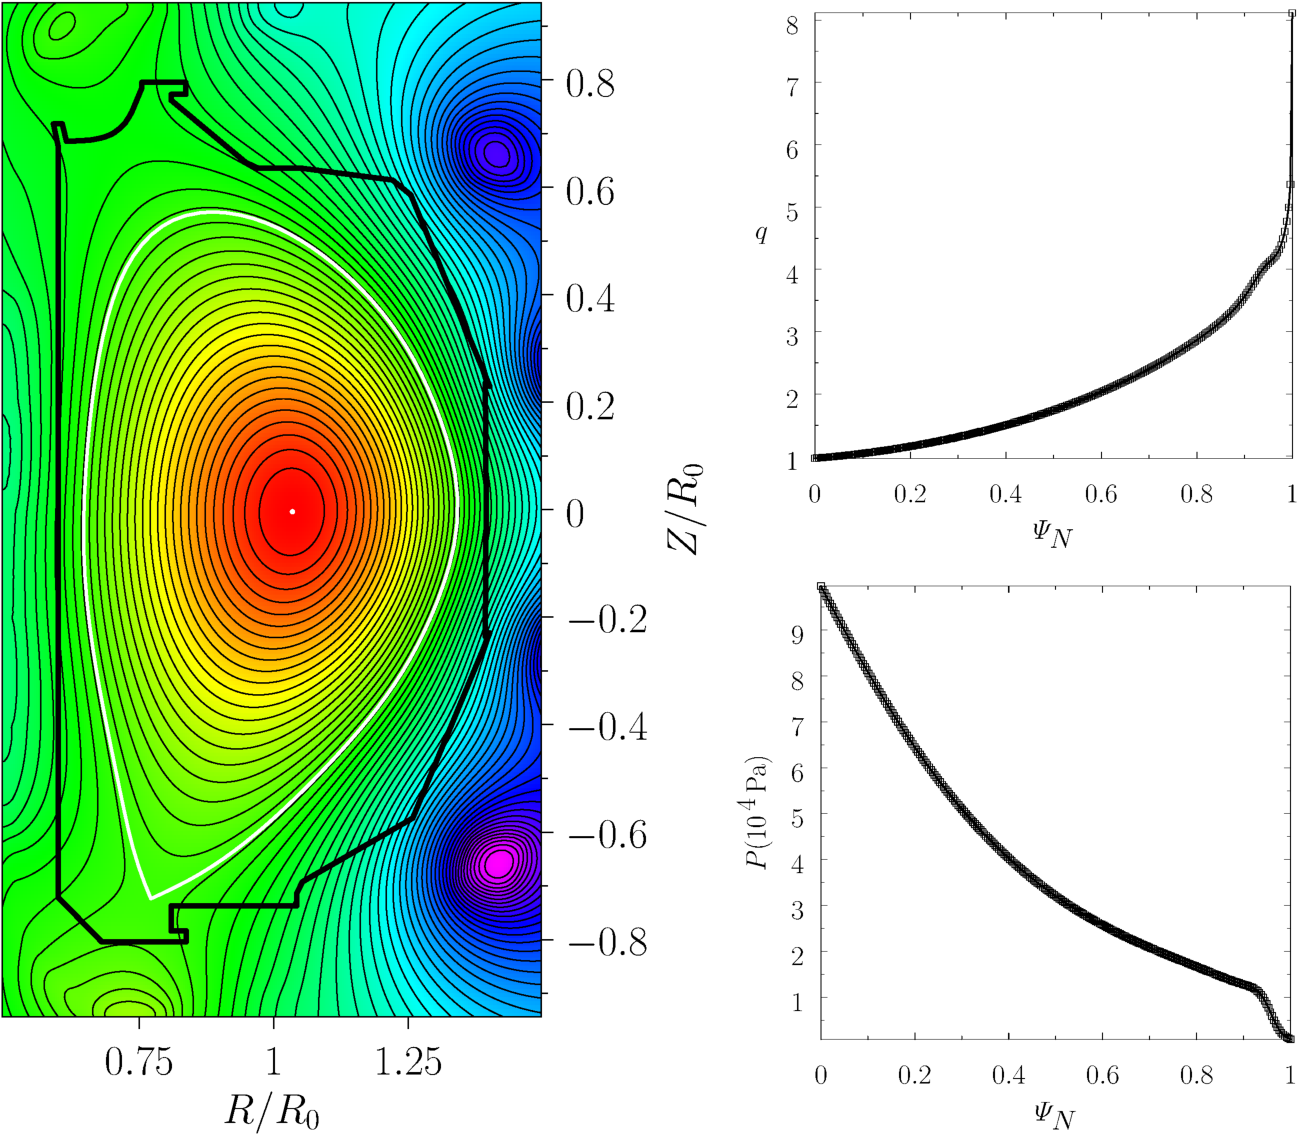
\includegraphics[height=6in]{fig2.pdf}
%\caption{}
%\end{figure}
\end{document}